\documentclass[11pt,a4j]{jsarticle}

\usepackage{float,array,booktabs,here}
\usepackage{amsmath}
\usepackage[dvipdfmx]{graphicx}
\usepackage[top=20truemm,bottom=25truemm,left=20truemm,right=20truemm]{geometry}
\usepackage{url}

\makeatletter
\newcommand{\figcaption}[1]{\def\@captype{figure}\caption{#1}}
\newcommand{\tblcaption}[1]{\def\@captype{table}\caption{#1}}
\makeatother

\newcommand{\Maru}[1]{\ooalign{
\ifnum#1<10 \hfil\resizebox{.9\width}{.85\height}{#1}\hfil
\else
\hfil\resizebox{.6\width}{.8\height}{#1}\hfil
\fi
\crcr
\raise.1ex\hbox{$\bigcirc$}}}


\begin{document}

\title{マイクロプロセッサ}
\author{hogehoge}
\maketitle





\section{外部仕様}
\label{sec:外部仕様}

\subsection{概要}
\label{sub:概要}

モグラ叩きゲームを作成した。
難易度は3種類あり、選択してからゲームをスタートする。
制限時間は20秒であり、ゲーム終了後に3位までのハイスコアが表示される。
プレーヤーが3位までのスコアを上回った場合、メッセージが表示される。

\subsection{実験装置}
\label{sub:実験装置}
実験に使用したFPGAボードと液晶モニタ、拡張ボードを図\ref{fig:machine}に示す。

\begin{figure}[H]
  \centering
  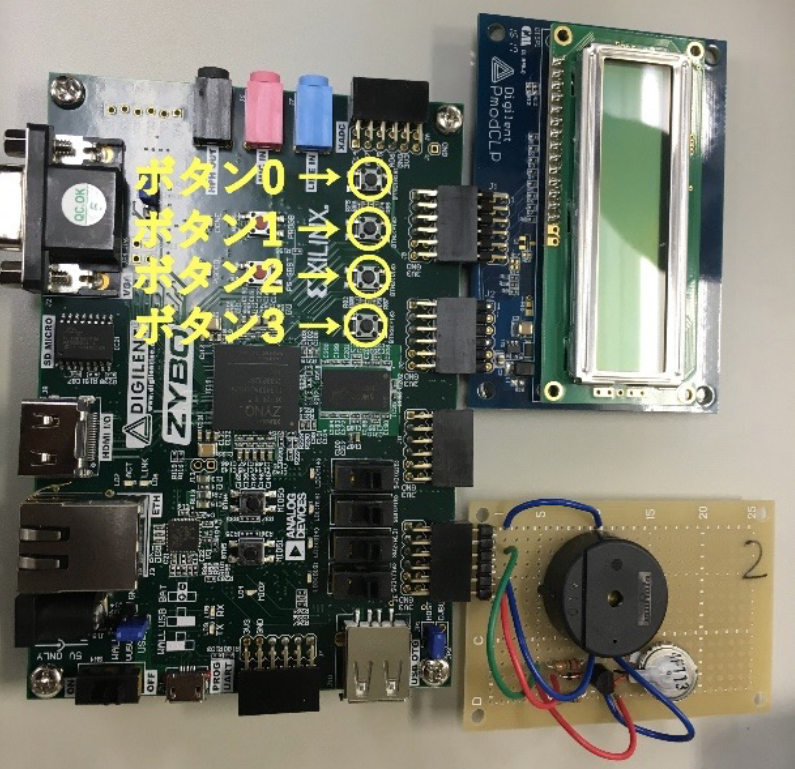
\includegraphics[height=60mm,bb=0 0 795 769]{img/machine.png}
  \figcaption{実験装置}
  \label{fig:machine}
\end{figure}

ゲームに使用するボタンを図\ref{fig:machine}のようにボタン0~3とした。

\subsection{ゲームの進め方}
\label{sub:ゲームの進め方}

まず、図\ref{fig:start}のようなスタート画面が表示される。

\begin{figure}[H]
  \centering
  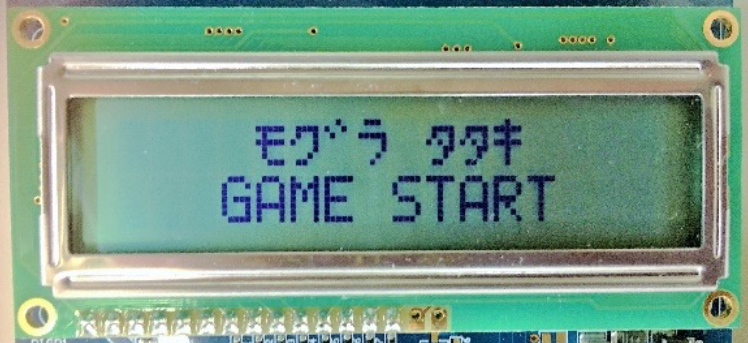
\includegraphics[height=25mm,bb=0 0 748 343]{img/start.png}
  \figcaption{スタート画面}
  \label{fig:start}
\end{figure}

次に難易度を3種類から選択する。

\begin{figure}[H]
  \centering
  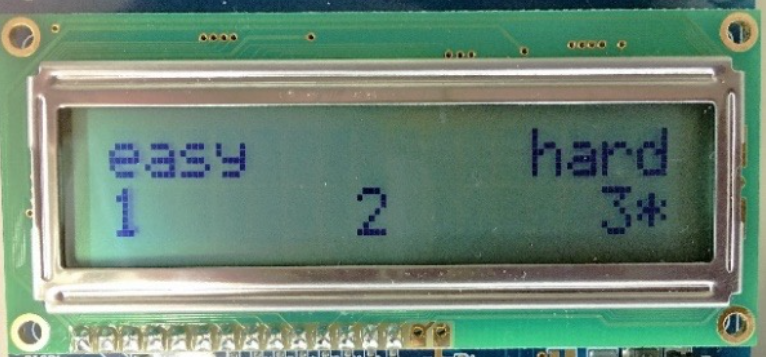
\includegraphics[height=25mm,bb=0 0 748 343]{img/select_mode.png}
  \figcaption{難易度選択画面}
  \label{fig:select}
\end{figure}

モード1が最も容易であり、モード3が最も難しい。
ボタン0でカーソルを左に、ボタン2でカーソルを右に移動する。
ボタン1で決定するとゲームがスタートする。

\begin{figure}[H]
  \centering
  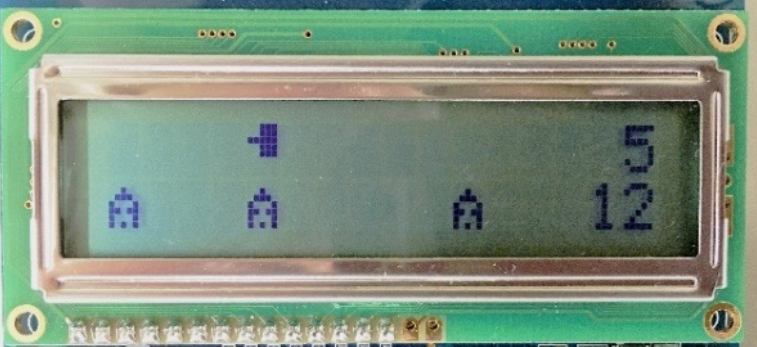
\includegraphics[height=25mm,bb=0 0 757 347]{img/play.png}
  \figcaption{プレイ画面}
  \label{fig:play}
\end{figure}

図\ref{fig:play}はゲーム中の画面である。
制限時間は20秒であり、画面右上にはスコアが、右下には残り時間が表示されている。
ボタン0でハンマーを左に、ボタン2でハンマーを右に移動し、ボタン1でモグラを叩く。
モグラを叩くとスコアが1ずつ増えていき、ブザーが鳴る。ミスした場合モータが振動するが、スコアは変化しない。


\begin{figure}[H]
  \centering
  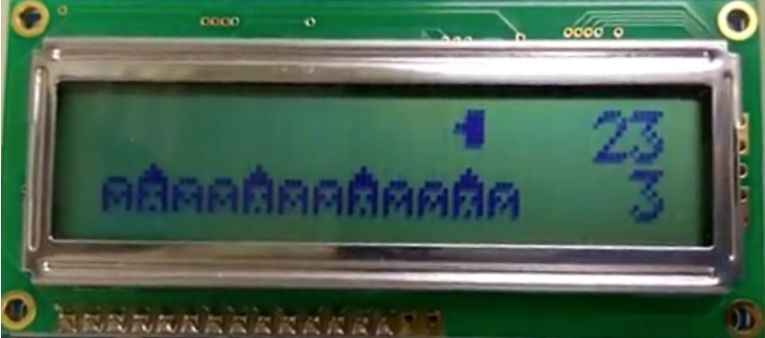
\includegraphics[height=25mm,bb=0 0 765 338]{img/feaver.png}
  \figcaption{フィーバータイム}
  \label{fig:feaver}
\end{figure}

残り時間3秒になった時にスコアが15以上であると、フィーバータイムとなり図\ref{fig:feaver}のようにボスモグラが出現する。
ボスモグラ出現時はハンマーがどこの位置にあってもボタン1を押すことでスコアを増やすことができる。

\begin{figure}[H]
  \centering
  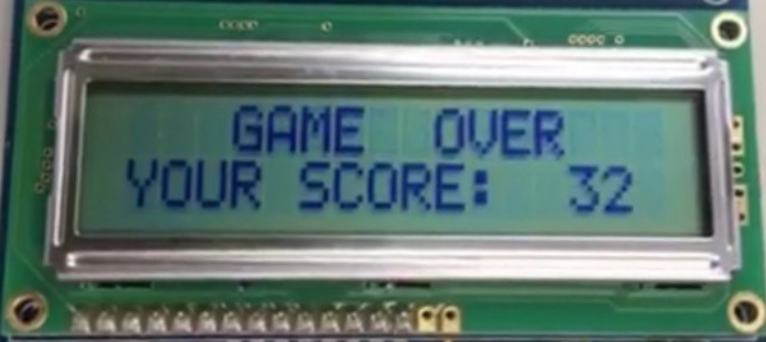
\includegraphics[height=25mm,bb=0 0 766 342]{img/result.png}
  \figcaption{結果の表示}
  \label{fig:result}
\end{figure}

\begin{figure}[H]
  \centering
  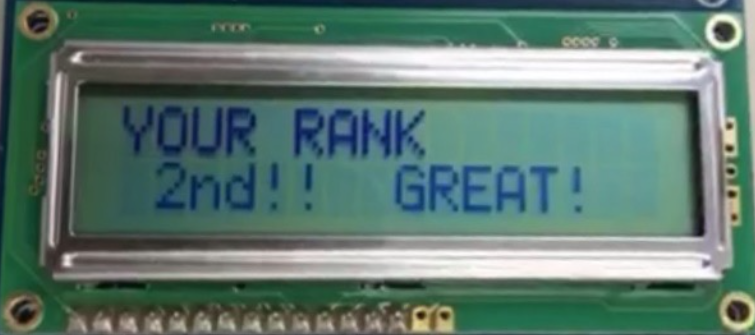
\includegraphics[height=25mm,bb=0 0 755 335]{img/update.png}
  \figcaption{ランキングの更新の表示}
  \label{fig:update}
\end{figure}

残り時間が0になるとゲームが終了し、図\ref{fig:result}のようにスコアが表示される。
スコアが3位までのハイスコアを上回っている場合、図\ref{fig:update}のようにメッセージが表示される。

\begin{figure}[H]
  \centering
  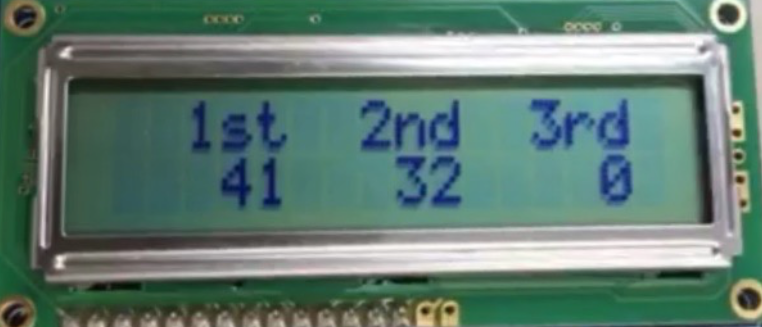
\includegraphics[height=25mm,bb=0 0 762 327]{img/ranking.png}
  \figcaption{ランキングの表示}
  \label{fig:ranking}
\end{figure}

その後、図\ref{fig:ranking}のように3位までのスコアのランキングが表示される。


\begin{figure}[H]
  \centering
  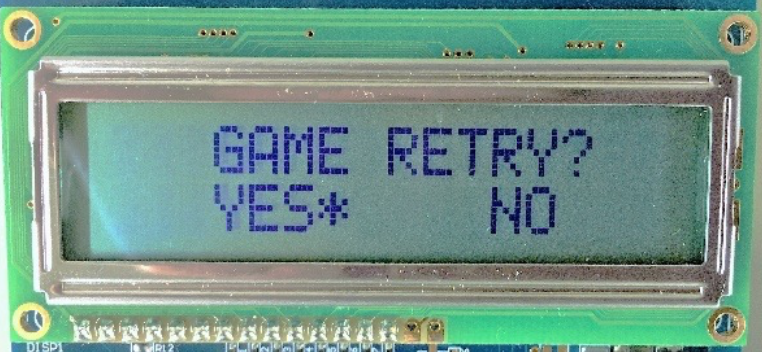
\includegraphics[height=25mm,bb=0 0 762 352]{img/retry.png}
  \figcaption{リトライの確認}
  \label{fig:retry}
\end{figure}

最後にリトライするかどうかの選択画面が表示される。
ボタン0とボタン2を用いてカーソルを動かし、ボタン1で決定する。
YESを選択すると同じモードでリトライすることができ、再びプレイ画面が表示される。


\section{内部仕様}
\label{sec:内部仕様}

\subsection{概要}
\label{sub:概要}

内部仕様は以下の図\ref{fig:flow}のようなフローチャートで表される。

\begin{figure}[H]
  \centering
  \includegraphics[height=210mm,bb=0 0 4408 13975]{img/mogura.png}
  \figcaption{内部仕様のフローチャート}
  \label{fig:flow}
\end{figure}


\end{document}
